% SPDX-License-Identifier: CC-BY-4.0
% SPDX-FileCopyrightText: 2026 Dan C. Hsu and Luke Lu
% Repository rendering of the GRACE paper figure: https://arxiv.org/abs/2607.09175
\documentclass[tikz,border=3pt]{standalone}
\usepackage{xcolor}
\usepackage{amsmath}
\usetikzlibrary{arrows.meta,shapes.geometric}

\definecolor{graceblue}{HTML}{3B5794}
\definecolor{ablorange}{HTML}{7E8DB9}
\definecolor{hcered}{HTML}{E64B35}

\begin{document}
\pagecolor{white}
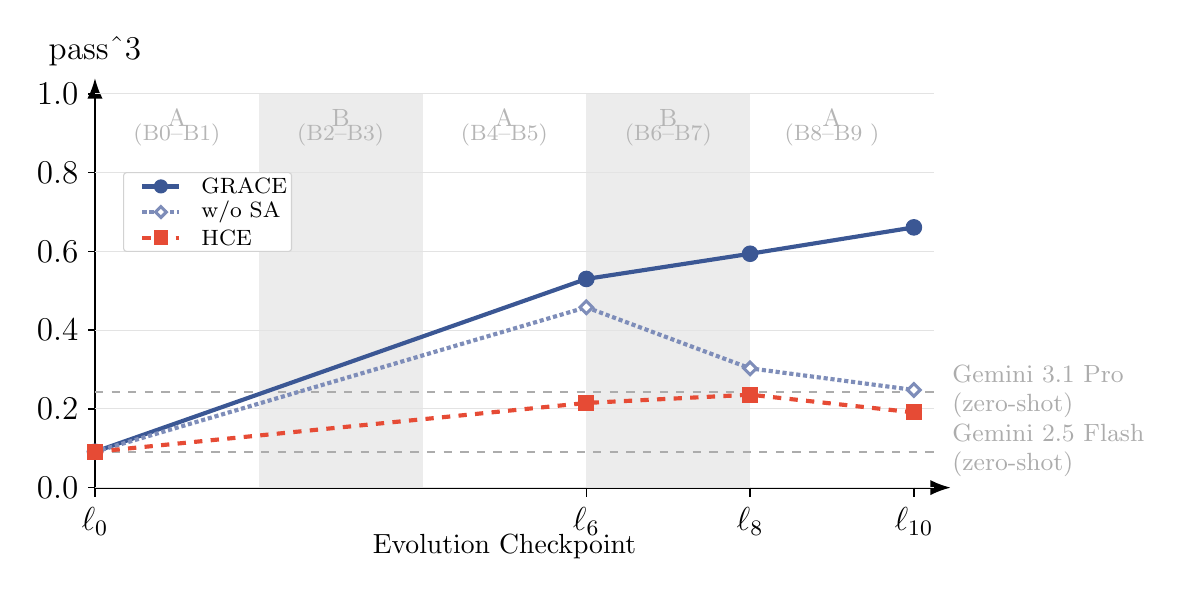
\begin{tikzpicture}[x=1.04cm,y=5.0cm]
  \fill[gray!15] (2,0) rectangle (4,1.0);
  \fill[gray!15] (6,0) rectangle (8,1.0);

  \foreach \x/\phase/\batches in {
    1/A/{B0--B1},
    3/B/{B2--B3},
    5/A/{B4--B5},
    7/B/{B6--B7},
    9/A/{B8--B9}
  } {
    \node[gray!58] at (\x,0.94) {\small \phase};
    \node[gray!58] at (\x,0.895) {\footnotesize (\batches)};
  }

  \draw[-{Latex[length=2.6mm]},line width=0.7pt] (0,0) -- (10.45,0);
  \draw[-{Latex[length=2.6mm]},line width=0.7pt] (0,0) -- (0,1.04);
  \node[anchor=south] at (0,1.045) {\large pass\textasciicircum{}3};
  \node at (5,-0.15) {\normalsize Evolution Checkpoint};

  \foreach \y/\label in {0/0.0,0.2/0.2,0.4/0.4,0.6/0.6,0.8/0.8,1.0/1.0} {
    \draw[gray!22,line width=0.35pt] (0,\y) -- (10.25,\y);
    \draw[line width=0.55pt] (0,\y) -- (-0.08,\y) node[left] {\large \label};
  }

  \foreach \x/\label in {
    0/$\ell_0$,
    6/$\ell_6$,
    8/$\ell_8$,
    10/$\ell_{10}$
  } {
    \draw[line width=0.55pt] (\x,0) -- (\x,-0.025) node[below] {\large \label};
  }

  \draw[gray!65,dashed,line width=0.75pt] (0,0.242) -- (10.25,0.242);
  \node[gray!65,anchor=west,align=left] at (10.35,0.245)
    {\small Gemini 3.1 Pro\\[-0.15em]\small (zero-shot)};
  \draw[gray!65,dashed,line width=0.75pt] (0,0.091) -- (10.25,0.091);
  \node[gray!65,anchor=west,align=left] at (10.35,0.095)
    {\small Gemini 2.5 Flash\\[-0.15em]\small (zero-shot)};

  \draw[graceblue,line width=1.5pt] (0,0.091) -- (6,0.530) -- (8,0.594) -- (10,0.661);
  \draw[ablorange,densely dotted,line width=1.5pt] (0,0.091) -- (6,0.458) -- (8,0.303) -- (10,0.248);
  \draw[hcered,dashed,line width=1.5pt] (0,0.091) -- (6,0.215) -- (8,0.236) -- (10,0.191);

  \foreach \x/\y in {0/0.091,6/0.530,8/0.594,10/0.661} {
    \draw[graceblue,fill=graceblue] (\x,\y) circle (2.8pt);
  }
  \foreach \x/\y in {0/0.091,6/0.458,8/0.303,10/0.248} {
    \node[diamond,draw=ablorange,fill=white,line width=1.1pt,inner sep=1.25pt] at (\x,\y) {};
  }
  \foreach \x/\y in {0/0.091,6/0.215,8/0.236,10/0.191} {
    \node[rectangle,draw=hcered,fill=hcered,minimum size=5.4pt,inner sep=0pt] at (\x,\y) {};
  }

  \draw[fill=white,draw=gray!35,rounded corners=1pt] (0.35,0.60) rectangle (2.40,0.80);
  \draw[graceblue,line width=1.5pt] (0.58,0.765) -- (1.03,0.765);
  \draw[graceblue,fill=graceblue] (0.805,0.765) circle (2.35pt);
  \node[anchor=west] at (1.18,0.765) {\footnotesize GRACE};
  \draw[ablorange,densely dotted,line width=1.5pt] (0.58,0.700) -- (1.03,0.700);
  \node[diamond,draw=ablorange,fill=white,line width=1.1pt,inner sep=1.1pt] at (0.805,0.700) {};
  \node[anchor=west] at (1.18,0.700) {\footnotesize w/o SA};
  \draw[hcered,dashed,line width=1.5pt] (0.58,0.635) -- (1.03,0.635);
  \node[rectangle,draw=hcered,fill=hcered,minimum size=4.9pt,inner sep=0pt] at (0.805,0.635) {};
  \node[anchor=west] at (1.18,0.635) {\footnotesize HCE};
\end{tikzpicture}
\end{document}
